\documentclass[UTF8,a4paper]{ctexart}
\usepackage[margin=1in]{geometry}
\usepackage{graphicx,float,array,color}
\author{qhy}
\date{\today}
\title{ML Note}
\begin{document}
    \maketitle
    \tableofcontents
    \newpage
    \section{SVM}
    定义标签:$\hat{y} = \{+1,-1\}$,+1表示正类,-1表示负类
    定义输出:
    \begin{equation}
        g(x) = \left \{
            \begin{array}{ll}
                +1 & ,f(x) > 0 \\
                -1  & ,f(x) >0
            \end{array} \right .
    \end{equation}

    定义loss functon:
    \begin{equation}
        L(f) = \sum_n I(g(x^n \neq \hat{y}^n))
    \end{equation}

    也就是统计分类错误的个数,从更一般的角度来看,就是每分类错误一个,就给一定的惩罚

    分析:$\hat{y^n}f(x^n)>0$的时候,分类正确,无论是正类还是负类,

    如果把这个看做一个新的变量t,那么损失函数(一个数据的损失函数)就可以定义成$t>0$时无惩罚,$t<0$的时候给出一定的惩罚。

    \begin{figure}[H]
        \centering
        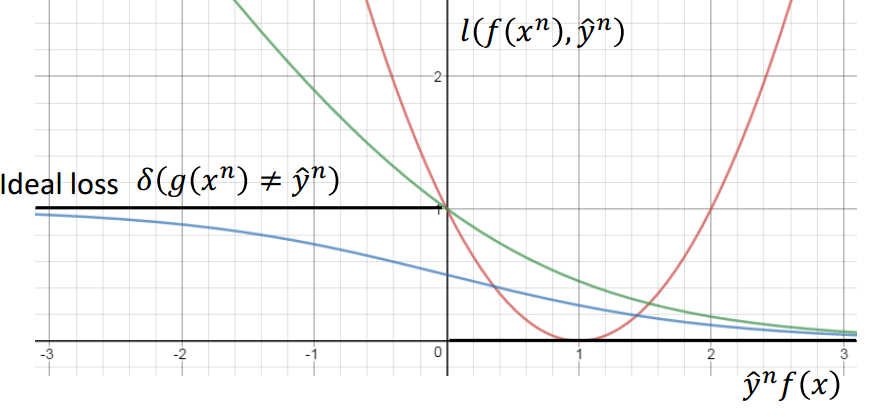
\includegraphics[scale = 0.3]{assets/ML_1a136.png}
        \label{figlossfunction}
    \end{figure}

    理想的情况就是图\ref{figlossfunction}中的黑线,分类错误就给出惩罚。

    由于此loss function使用梯度下降算法麻烦,故使用一个惩罚函数l代替I:
    \begin{equation}
        L(f) = \sum_n I(f(x^n , \hat y^n))
    \end{equation}

    红色线为\textbf{Square loss}:
    \begin{equation}
        l(f(x^n , \hat y^n) = (\hat y^n f(x^n) - 1)^2
    \end{equation}
    显然是不合理的,因为它对于分类正确的结果也给出了惩罚。

    蓝色线为\textbf{sigmoid+ square loss}:
    \begin{equation}
        l(f(x^n , \hat y^n) = (\sigma(\hat y^n f(x^n)) - 1)^2
    \end{equation}
    这样,得到的结果是合理的,对于分类正确,确定性高的给出低惩罚,对于分类错误,甚至错误的离谱的,则给出大的惩罚

    但是有一个问题就是,对于分类错误的结果,它的惩罚很低。

    绿色线为\textbf{Sigmoid + cross entropy}
    \begin{equation}
        l(f(x^n , \hat y^n) = \ln(1 + exp(-y^n f(x^n)))
    \end{equation}

    蓝色线为\textbf{hinge loss}:
    \begin{equation}
        l(f(x^n , \hat y^n) = max(0, 1 - y^n f(x^n))
    \end{equation}

    对于分类正确的结果,只要$yf(x) < 1$的数据还是会给出惩罚,而SVM采用的就是$Hinge Loss$

    从$f(x)$来看,$f(x)$为分界线,只要在$f(x)$上下距离为1的样本都会给出惩罚。

        \subsection{线性SVM}
        模型如下:
        \begin{figure}[H]
            \centering
            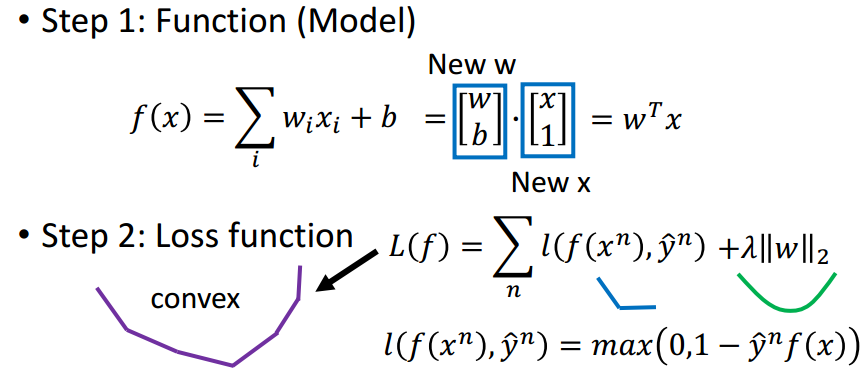
\includegraphics[scale = 0.3]{assets/ML_2f26e.png}
            \label{figlinearSVM}
        \end{figure}

        梯度下降:
        \begin{figure}[H]
            \centering
            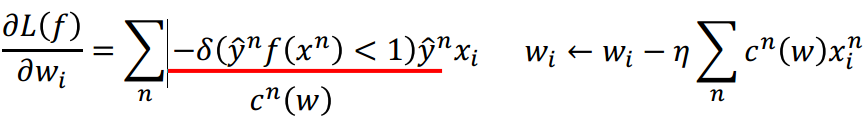
\includegraphics[scale = 0.3]{assets/ML_b932f.png}
            \label{figlinearSVMGradientDescent}
        \end{figure}

        \subsection{线性SVM2}
        {\color{red} 至此,线性SVM结束,但是这个SVM和之前见到的SVM貌似不太一样?对偶问题,SMO,等等这些东东呢?}

        另一种描述:
        \begin{figure}[H]
            \centering
            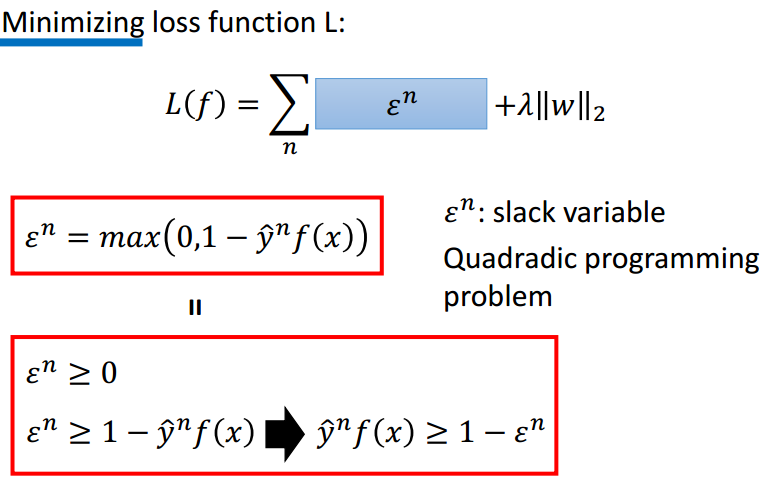
\includegraphics[scale = 0.3]{assets/ML_e1a0b.png}
        \end{figure}

        经过这样处理,原问题从
        最小化:
        \begin{figure}[H]
            \centering
            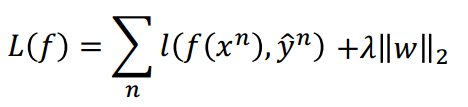
\includegraphics[scale = 0.3]{assets/ML_5215d.png}
        \end{figure}

        变成了最小化:
        \begin{figure}[H]
            \centering
            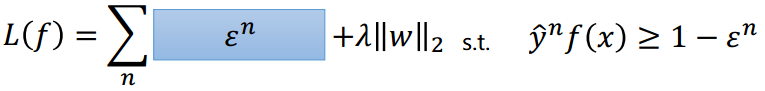
\includegraphics[scale = 0.3]{assets/ML_a74a0.png}
        \end{figure}

        进一步处理,问题变成最小化:
        \begin{figure}[H]
            \centering
            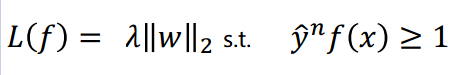
\includegraphics[scale = 0.3]{assets/ML_371e4.png}
        \end{figure}












\end{document}
